\documentclass[csgeo,tcc]{unipampa}                                          
\usepackage[utf8]{inputenc} 
\usepackage[T1]{fontenc}                                    
\usepackage{graphicx}                                       % pacote para importar figuras
\usepackage{chngcntr}                                       % pacote que permite a mudança da contagem das figuras e tabelas
\counterwithout{figure}{chapter}                            % contagem contínua das figuras [Não especificado nas normas, porém de preferência do autor]
\usepackage{times}                                          % pacote para usar fonte Adobe Times

\usepackage{mathptmx}                                       % pacote usar fonte Adobe Times nas fórmulas
\usepackage[alf,abnt-emphasize=bf]{abntex2cite}	           % pacote para usar citações abnt
\usepackage{ragged2e}                                       % pacote para prevenir hifenização e melhorar disposição de objetos
%\hyphenpenalty=10000                                        % penalização de hifenização, força texto justificado
\usepackage{booktabs}                                       % pacote que melhora a qualidade das tabelas geradas pelo LaTeX
\usepackage[table]{xcolor}                                  % pacote para utlização de cores personalizadas
\usepackage[labelsep=endash]{caption}                       % pacote para customização de títulos ou legendas de figuras 
\usepackage{amsmath}
\usepackage{xcolor}
\usepackage{verbatim}

% ATALHOS =================================================================================================================

\newcommand{\rot}[1]{\nabla \times \textrm{#1}}
\newcommand{\MT}{magnetotelúrico }                                              % mt -> magnetotelúrico
\newcommand{\citar}[1]{\textcolor{red}{#1}}                                     % marca em vermelho locais para correção
\newcommand{\en}[1]{\textit{#1}}                                                % marca em italico termos em ingles



% ATALHOS PARA CODIGO FONTE
\newcommand{\codnum}[1]{\begin{flushright} \normalsize (#1) \end{flushright}}   %numera os scripts
\newcommand{\codbox}[1]{{\fontfamily{pcr}\selectfont #1}}                       %ambiente para escrever codigo fonte. OBS deve estar dentro do ambiente quote
\newcommand{\cc}[1]{\textcolor{gray}{\textit{\# #1}}}                           %cor para comentarios (cinza)
\newcommand{\f}[1]{\textbf{\textcolor{OliveGreen}{#1}}}                         %cor para funcoes (verde)
\newcommand{\cl}[1]{\textbf{\textcolor{BurntOrange}{#1}}}                       %cor para classes (laranja)
\newcommand{\ob}[1]{\textcolor{Blue}{#1}}
\newcommand{\st}[1]{\textcolor{OliveGreen}{#1}}
\newcommand{\ini}{>{}>{}> \, }                                                  % produz >>>
\newcommand{\init}{>{}>{}> \, \, \, \, \,}                                      % produz >>> tabulado 1vez
%\newcommand{\init2}{>{}>{}> \, \, \, \, \, \, \, \, \,}                        % produz >>> tabulado 2vez
%\newcommand{\init3}{>{}>{}> \, \, \, \, \, \, \, \, \, \, \, \, \,}            % produz >>> tabulado 3vez






% =========================================================================================================================





% TITULO, AUTOR, ORIENTADOR =============================================================================================== 

% TITULO
	\title{Desenvolvimento de Software livre para processamentos de Dados Magnetotelúricos}                              

% AUTOR
	\author{Garcia}{Patrick Rogger}                                    

% ORIENTAÇÃO
	\advisor[Prof.~Dr.]{Oliveira}{Vinicius Abreu de}                        
	\coadvisor[Prof\textsuperscript{a}.~Dr.\textsuperscript{a}.]{Matos}{Andréa Cristina Lima dos Santos}   
	\renewcommand{\coadvisorname}{Co-orientadora}
% =========================================================================================================================






% BANCA ===========================================================================================================

% BIBLIOTECA
	\cutter{} 
% MEMBRO 1
	\banca[Prof.~Dr.]{SOBRENOME}{NOME}			                
	\inst{Universidade Federal do Pampa}					    

% MEMBRO 2
	\banca[Prof.~Dr.]{SOBRENOME}{NOME}                           
	\inst{Universidade Federal do Pampa}	                    

% DATA DA DEFERSA
	\defesa{DIA}{MÊS}{ANO}                                    
% ====================================================================================================================








% DATA E LOCAL =======================================================================================================
% SE PRECISAO MUDAR A DATA DO DOCUMENTO
	%\date{MÊS}{ANO}
% LOCAL
	\location{Caçapava do Sul}{RS}                              
% =====================================================================================================================








% PALAVRAS CHAVES =====================================================================================================
	\keyword{Kivy}	
	\keyword{Magnetotelúrico}
	\keyword{Python3}
	\keyword{Software Livre}
% ======================================================================================================================








% CORRIGIR TEXTO =======================================================================================================
	\sloppy                                                       
% ======================================================================================================================








% DOCUMENTO ============================================================================================================
\begin{document}
\maketitle






% DEDICATORIA ==========================================================================================================

	%\begin{dedicatoria} 
	%	
	%\end{dedicatoria}
% =======================================================================================================================








% AGRADECIMENTOS ========================================================================================================
	
	%\chapter*{Agradecimento}
	% 
% ========================================================================================================================







% EPIGRADE ================================================================================================================
	%\begin{epigrafe}
	%	``Moça bonita, moça bem feita.''\\
	%	--- Sr. Madruga
	%\end{epigrafe}
% ========================================================================================================================








% RESUMO ===============================================================================================================

%	\begin{abstract} 
%		Escreva aqui seu resumo em português. 		
%	\end{abstract}
% =========================================================================================================================







% RESUMO EM INGLES ========================================================================================================
%	\begin{englishabstract}
%		Escreva aqui seu resumo em língua estrangeira.
%	\end{englishabstract}

% ==========================================================================================================================







% LISTA DE FIGURA E TABELA =================================================================================================

\listoffigures
\listoftables
% ==========================================================================================================================






%  LISTA DE TEOREMAS ==========================================================================================================================
% Listas de definições e teoremas, para quem usar o pacote formais, para trabalhos que possuam definições formais e teoremas

%\listofdefinitions
%\listoftheorems
% ==========================================================================================================================






% LISTA DE ABREVIATURAS ====================================================================================================

%\begin{listofabbrv}{UNIPAMPA}
        
%        \item[SIGLA]{NOMECOMPLETO}        
%        \item[SIGLA]{NOMECOMPLETO}         
      
%\end{listofabbrv}
% =============================================================================================================================







% LISTA DE SIMBOLOS ===========================================================================================================

%\begin{listofsymbols}{$\alpha\beta\pi\omega$}
%       \item[$\rho$]          			  Resistividade
%       \item[$\nabla$]    				  Nabla
%       \item[$\rot{B}$]					  Mag
       
%\end{listofsymbols}
% =============================================================================================================================







% SUMARIO ==================================================================================================================
\tableofcontents
% ==========================================================================================================================







% CORPO DO TEXTO ===============================================================================================================
\inputencoding{utf8}                                %% Arquivos em outra codificação: UTF-8

% CAPITULO 1 ===================================================================================================================
	% INTRODUÇÃO


\chapter{Introdução \,\,\,\,\,\,\,\,\ OK}
    \label{cap-introducao}
    
	Apoiado nas leis de Maxwell o método MT (Magnetotelúrico) usa a Terra como 
	um condutor ôhmico e as variações do seu campo 
	magnético promovido por ventos solares \cite{parkinson93} e tempestades equatoriais 
	que interagem com a ionosfera para investigar as 
	estruturas internas da Terra e litologias rasas. 
	
	
	No Brasil o uso do método MT é insipiente, restrito ao meio acadêmico e pouco
	utilizado na indústria, porém, pode ser bem aplicado na prospecção de 
	hidrocarbonetos, sendo a sua resolução melhor que a magnetometria
	e gravimetria, também em estudos crustais
	apoiando a sismologia devido sua grande profundidade de investigação, mas o 
	alto custo de processamento e a falta de \textit{softwares} para trabalhar com os 
	dados tem sido algumas das causas do fraco uso.
	
	
	Esse trabalho foi pensado primeiramente para tornar o MT mais difundido, 
	construindo um \textit{software} com interface gráfica e 
	distribuição livre. O \textit{software} então nasceu 
	com esse propósito, compreendendo o processamento de dados
	MT desde a coleta até a primeira visualização dos dados, como: escolha 
	de bandas, plotagem de pseudo-secções em função de resistividade e fase 
	também fazendo tratamentos estatísticos e processamento robusto 
	proposto por \citeauthor{egbert97} \citeyearpar{egbert97}.
	
	
	O programa será construído usando a linguagem Python \cite{python36} 
	e a construção da interface gráfica será desenvolvida usando a API
	Kivy \cite{kivy110} dentre outros pacotes. A escolha por essa linguagem foi a vasta quantidade de pacotes,  o crescente 
	número de pessoas implementando e a facilidade da construção do código.






% CAPITULO 2 ===================================================================================================================
	
\chapter{Objetivos \, \,\,\,\,\, OK}
\label{cap-objetivos}

\section{Objetivos Gerais}
\label{cap-objetivos gerais}

    
    O objeto de estudo desse trabalho é o desenvolvimento de um \en{Software} para tratamentos e processamentos de dados \MT, também a aplicação do programa no processamento e comparação de dados reais coletados em uma região do nordeste brasileiro, conhecida como província Borborema, região que vem sendo grandemente estudada com o \MT e proporciona a este trabalho boa validação dos algoritmos de processamento.

\section{Objetivos Específicos}
\label{cap-objetivos especificos}

    O MT é um método geofísico que trabalha com propriedades eletromagnéticas, essa característica torna o processamento dos dados extremamente trabalhoso e com alto custo computacional, o trabalho então propõe a criação de novos algoritmos e otimização dos que já existem para tornar o processamento mais fácil e barato.
    
    Tem objetivo também de obter pseudosecções de resistividades e modelos lito-geofísicos de resistividade para a região de estudo com as novas rotinas comparando com trabalhos anteriores \cite{tese_andrea} e \cite{alane}.

	\chapter{Justificativa}
\label{cap-justificativa}

    Esse trabalho foi pensado para auxiliar a expansão do \MT, hoje existem vários programas proprietários para processamento destes tipos de dados, mas, são programas de alto custo e fechados, isto é, não possuem transparência dos fluxos de processamentos dentro do programa. O processamento hoje usado na maioria dos trabalhos usam como base os algoritmos propostos por \citeauthor{egbert97} para a primeira fase de processamento e a rotina To Jones \cite{egbert97} para compilação dos dados em arquivos manipuláveis.
    
    Esses processos atualmente são feitos através de linhas de comando unindo diversos programas separados, o que torna o procedimento muito instável provocando diversos tipos de erros além de não prever outros. %Também força a instalação de vários pacotes separados que muitas vezes são compilados e instalados manualmente, afastando uma pessoa leiga em computação a utilizar.
    
    O programa proposto aqui pretende ser escrito em apenas uma linguagem e utilizar pacotes nativamente compatíveis, o que prevê erros de compatibilidades e torna a manutenção do código mais fácil uma vez que os códigos não serão compilados.
    
    Outra forma de beneficiar a utilização do programa será a construção de uma interface gráfica para todos os processos, tornando assim mais fácil utilizar prevenir erros provocados pelo usuário.    
    
    

	\chapter{Materiais e Métodos}
    \label{cap-materiais}    
    
    O método \MT proposto por \citeauthor{tikhonov50} \citeyearpar{tikhonov50} e
    \citeauthor{cagniard53} \citeyearpar{cagniard53}, usa as propriedades
    eletromagnéticas para estudar a distribuição de resistividade na crosta, 
    podendo variar a sua investigação de dezenas de metros a dezenas de 
    quilômetros.
    
    \section{Origem das Correntes Telúricas}
    
    As flutuações no campo magnético terrestre geram campos elétricos na alta atmosfera que induzem correntes magnéticas, as ondas eletromagnéticas então penetram no interior da Terra na forma de ondas planas ortogonais que induzem novas correntes chamadas de corrente telúricas que trazem informações das características físicas das litologias. 
    
    Uma das características é a modulação da frequência, causada por diferentes tipos de rochas e estruturas, esse fenômeno é diretamente 
	relacionado a resistividade do meio.
    
    As frequências das ondas são baixas variando de 1 $mHz$ à 10 $kHz$, ondas com frequências menores que 1 $Hz$ tem origem nos ventos solares que interagem como o campo magnético terrestre, já ondas com frequências maiores de 1 $Hz$ são provocadas por tempestades equatoriais. Para o estudo do \MT são feitas as seguintes suposições:
    
    \begin{enumerate}
	    \item Ondas geradas na ionosfera, distantes o suficientes, penetram ortogonais à superfície da Terra.	    
	    \item A Terra se comporta como um condutor ôhmico.
	    \item A Terra é considerada um semi-espaço isotrópico.
	\end{enumerate}   
    
    
%RESISTIVIDADE ==============================================================================================================================================
    \section{Resistividade dos Materiais}
    
    Para o \MT a propriedade investigação e contraste é a condutividade ($\sigma$) ou resistividade ($\rho$) sendo essa o inverso da condutividade.
    A resistividade é uma propriedade particular de cada material, ou seja, a partir de uma resistividade podemos estimar a qual material ela pertence\footnote{Para os meios geológicos essa propriedade é representada por um intervalo de valores, devido as complexidades químicas e físicas das diferentes litologias.}.
    
    Em 1827, Georg Ohm verificou de forma empírica que aplicando uma diferença de potencial em um material esse gera uma resistência a passagem de corrente, essa relação é chamada de lei de Ohm (equação \ref{lei_de_ohm})\cite{eletromag8hayt}.
    
    \begin{equation}
     \label{lei_de_ohm}
     V = R i
    \end{equation}
    
    Onde $V$ é a diferença de potencial (V), $i$ é a corrente (A) e $R$ é a resistência ($\Omega$), materiais que obedecem essa lei são chamados de materiais ômicos, a Terra é considerada um material ôhmico, porem para a investigação geofísica a resistência não é uma propriedade viável, visto  que depende muito da geometria do problema, assim foi proposto a resistividade, onde, um mesmo material terá a sua resistividade igual independente da geometria.
    
    A resistividade então é definida pela \textcolor{red}{ que o material oferece para um comprimento (equação \ref{resistividade})........ mudar isso e colocar igual do livro}, a figura \ref{fig_resistividade} mostra um circuito para se obter a resistividade, sendo A a área ($m^2$), R a resistência ($\Omega$), L o comprimento ($m$) e $\rho$ a resistividade dada em $\Omega m$. 
    
    \begin{equation}
        \label{resistividade}
        \rho = \dfrac{R A}{L}\, \, \, ;\, \, \, \, \, \, \, \, \, \, \, \, \, \,  R = \dfrac{V}{i}
    \end{equation}
    
    
    \begin{figure}[h]
        \centering
        \caption{Arranjo para medir a resistividade ($\rho$) de um material}
        \centerline{\includegraphics[width=4cm]{texto/fig/resisti_telford.png}}
        \fonte{Adaptado \citeauthor{telford}, \citeyearpar{telford}}
        \label{fig_resistividade}
    \end{figure}
    
    A figura \ref{tabela_resistividade} mostra a distribuição de resistividade para diversos materiais geológicos. 
    Portanto podemos identificar a partir de um contexto geológico quais litologias pertence a cada resistividade encontrada, por exemplo, uma litologia que tenha resistividade em torno de  $100 \, \Omega m$ e outra com $3000 \, \Omega m $ pode ser caracterizada como um arenito e uma rocha ígnea respectivamente. 
    
    \begin{figure}[h]
        \centering
        \caption{Resistividade dos Materiais Geológicos}
        \centerline{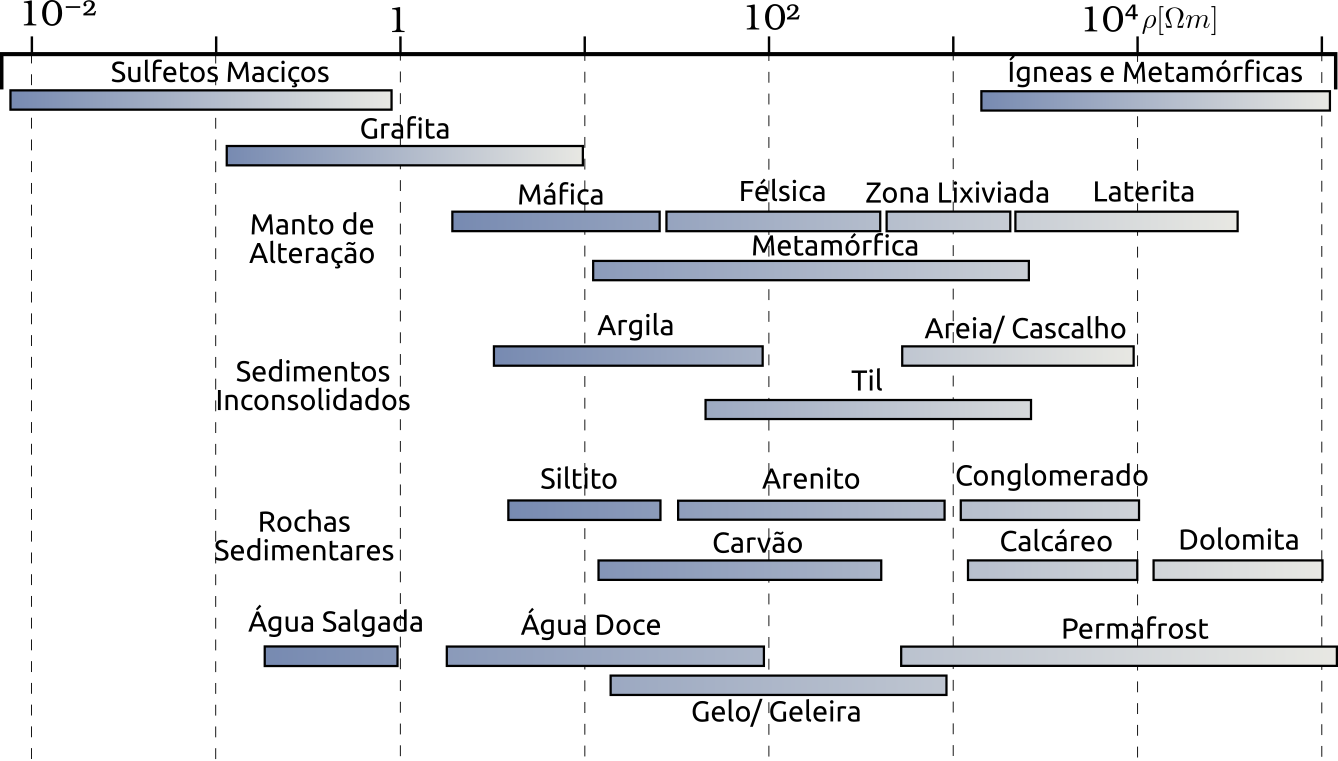
\includegraphics[width=14cm]{texto/fig/resistividade_tabela.png}}
        \fonte{Adaptado \citeauthor{eletromag_met}, \citeyearpar{eletromag_met}}
        \label{tabela_resistividade}
    \end{figure}
% FIM RESISTIVIDADE
%===========================================================================================================================================================    
    
    
    
% Eletromagneticos
%===================================================================================================================================================
    \section{Fundamentos Teóricos dos Métodos Eletromagnéticos}
        Usando as leis de Maxwell \cite{eletromag8hayt} podemos medir os campos elétricos e magnéticos e a partir deles estimar a resistividade dos meios litológicos em sub-superfície.
	
        Os campos podem ser descritos pelas seguintes equações\footnote{Para cargas e correntes livres
        (macroscópica)}:
            \begin{equation}
                \label{rot_elet_max}
                \nabla \times \vec{\textrm{E}}=-\frac{\partial \vec{\textrm{B}}}{\partial t} 
            \end{equation}
            \begin{equation}
                \label{rot_mag_max}
                \nabla \times \vec{\textrm{H}} = \vec{\textrm{J}} + \frac{\partial \vec{\textrm{D}}}{\partial t}
            \end{equation}
            \begin{equation}
                \nabla \cdot \vec{\textrm{B}} = 0
            \end{equation}
            \begin{equation}
                \nabla \cdot \vec{\textrm{D}} = \rho
            \end{equation}

            $\vec{\textrm{E}}$ $\rightarrow$ Campo Elétrico [$V/m$]
	    
            $\vec{\textrm{B}}$ $\rightarrow$ Campo Magnético [$T$]
	    
            $\vec{\textrm{H}}$ $\rightarrow$ Campo Magnetizante [$A/m$]
	    
            $\vec{\textrm{J}}$ $\rightarrow$ Densidade de Corrente [$A/m^2$]
	    
            $\vec{\textrm{D}}$ $\rightarrow$ Campo de Deslocamento Elétrico [$C/m^2$]
	    
            $\rho$ $\rightarrow$ Densidade de Carga [$C/m^3$]
	    
            $t$ $\rightarrow$ Tempo [$s$]

            Obedecendo as relações de contorno para um meio isotrópico temos as seguintes
            relações (equações constitutivas):
            \begin{equation}
                \label{con_B}
                \vec{\textrm{B}} = \mu \vec{\textrm{H}}
            \end{equation}
            \begin{equation}
                \label{con_D}
                \vec{\textrm{D}} = \varepsilon  \vec{\textrm{E}}
            \end{equation}
            \begin{equation}
                \label{con_J}
                \vec{\textrm{J}} = \sigma \vec{\textrm{E}}
            \end{equation}
	    
            $\mu$ $\rightarrow$ Permeabilidade Magnética [$H/m$]
	    
            $\varepsilon$ $\rightarrow$ Permissividade Elétrica [$F/m$]
	    
            $\sigma$ $\rightarrow$ Condutividade Elétrica [$S/m$]
	    
            Cada escalar das equações anteriores são características que dependem do meio em que a onda se propaga.
	    
            Para a crosta $\mu = 1,2566\textrm{x}10^{-6} H/m$ e $\varepsilon = 8,85
            \textrm{x}10^{-12} F/m$ esses parâmetros funcionam como tensores em um meio
            anisotrópico que variam em função do tempo, já considerando para os 
            trabalhos de investigação o meio supõe-se ser isotrópico, assim, 
            tornando estáticos os tensores.
	
    
    
    
    
    
% MT
%===================================================================================================================
    \section{Resposta do Método Magnetotelúrico}
        \subsection{Impedância Eletromagnética}
        
        
        
    
    
    
    \section{Modelo de Dimensões MT}
        \subsection{Terra 1D}
        \subsection{Terra 2D}
        
        O modelo de Terra 2D é caracterizado pelo contato vertical entre dois meios de diferentes resistividades. Se o contato é
	    paralelo ao eixo $x$ então é definido a direção do \textit{strike} no eixo $x$, a direção deve ser paralela ao plano de contato,
	    ou seja, onde a condutividade é constante.% (Figura \ref{fig_strike}).
	    
	    \begin{figure}[h]
	        \caption{Modelo de Terra 2D para a resistividade variando na direção $y$}
	        \begin{center}
	        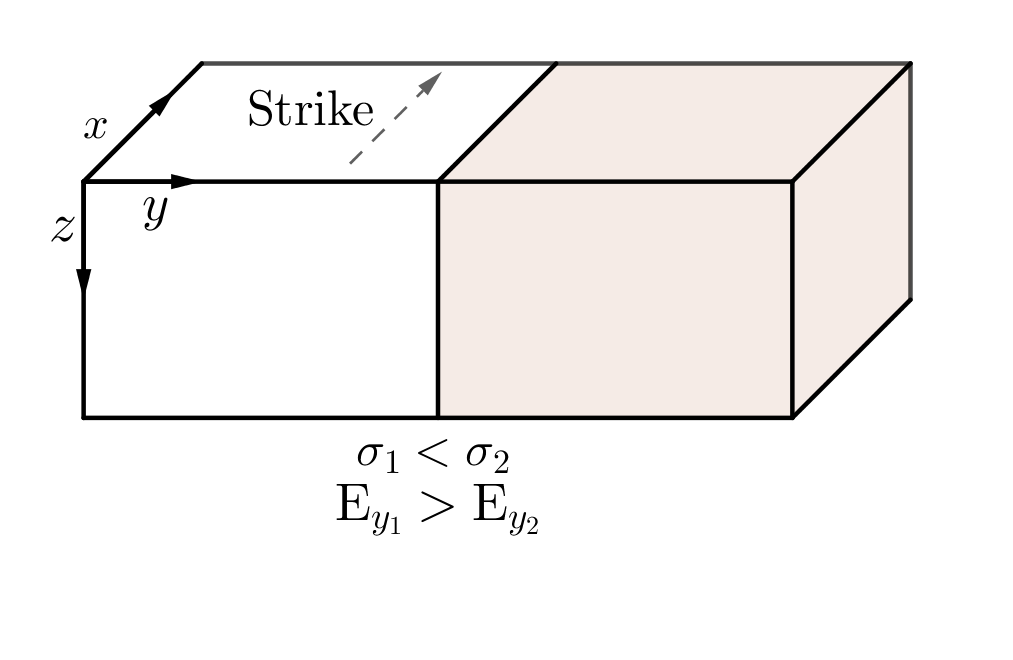
\includegraphics[width=12cm]{texto/fig/Tm_Te.png} 
	        \end{center}
		\fonte{Adaptado \cite{didana2010}}
		\label{fig_strike}
	    \end{figure}
	    Devido a essa diferença entre as resistividades polarizamos os campos em TE (Transversal Elétrico) e TM (Transversal Magnético).
	    Para esse modelo temos o tensor impedância como:
	    \begin{equation}
	     \textrm{Z}_{2D} = \left (\begin{array}{cc}
	                               0 & \textrm{Z}_{xy} \\
	                               \textrm{Z}_{yx} & 0
	                              \end{array} \right)
	    \end{equation}
	    Assim cada polarização pode ser escrita como:
	    \begin{equation}
	     \textrm{TE} = \left \{ \begin{array}{l}
	            \dfrac{\partial \textrm{E}_x}{\partial y} = \dfrac{\partial \textrm{B}_z}{\partial t} = -i\omega \textrm{B}_z \\
	           \dfrac{\partial \textrm{E}_x}{\partial z} = \dfrac{\partial \textrm{B}_y}{\partial t} = i\omega \textrm{B}_y \\
	           \dfrac{\partial \textrm{B}_z}{\partial y} - \dfrac{\partial \textrm{B}_y}{\partial z} = \mu \sigma \textrm{E}_x 
	           \end{array} \right.
	    \end{equation}
	    \begin{equation}
	     \textrm{TM} = \left \{ \begin{array}{l}
	            \dfrac{\partial \textrm{B}_x}{\partial y} = \mu \sigma \textrm{E}_z \\
	           -\dfrac{\partial \textrm{B}_x}{\partial z} = \mu \sigma \textrm{E}_y \\
	           \dfrac{\partial \textrm{E}_z}{\partial y} - \dfrac{\partial \textrm{E}_y}{\partial z} = i \omega \textrm{B}_x 
	           \end{array} \right.
	    \end{equation}
        
        
        \subsection{Terra 3D}
    
    \section{Processamento das Series Temporais (mudar o titulo)}
    
    \section{Ferramentas de Desenvolvimento do \textit{Software} \,\,\,\,\,\,\, OK}
    
        O desenvolvimento do \textit{software} foi baseado na filosofia de \textit{Software Livre} \cite{soft_free} onde o código fonte será liberado e distribuído para a comunidade geofísica. A linguagem base escolhida para o projeto foi o Python, visto as vastas bibliotecas para trabalhar com dados científicos e a simplicidade da implementação do código.  
        
        \subsection{Linguagem PYTHON}
            \label{lim_python}
            
            Criada nos anos 80 por Guido Van Rossum no CWI (\en{Centrum Wishunde \& Informatica}) em Amsterdã, Holanda a linguagem Python foi idealizada no grupo de desenvolvimento da linguagem ABC do CWI, rapidamente ela começou a ter destaque. Na década de 90 foi criada a \en{Python Software Activity} que começou a ser a mantenedora por exemplo do python.org, nesse período apenas o criador tomava decisões e era desenvolvedor da linguagem, finalmente em 2001 é fundada a \en{Python Software Foundation} que mantém a linguagem e todos os direitos sobre ela \cite{python36}.  
            
            Python é uma linguagem de alto nível onde seu código deve ser organizado favorecendo a interpretação ao mesmo tempo simples.
            
            Exemplos de código Python:

            Mostrar conteúdo na Tela:
            
            Como comentado, o código tem fácil leitura, para imprimir um conteúdo na tela 
            podemos simplesmente usar o comando \verb|print|, aproximando muito da linguagem falada.  
            \begin{quote}
             \codbox{\ini   \cc{Comentários}                  \\
                     \ini   \f{print} ('Hello World')          \\
                     Hello World
                     }                                          \codnum{\ref{lim_python}.1}

            \end{quote}
            
            Operações Matemáticas:
            
            As variáveis no código não precisam ser declaradas para um 
            tipo específico (Ex.: \textit{float, int, string}), deixando assim o código mais fluido. 
            \begin{quote}
            
             \codbox{\ini a = 2                               \\
                     \ini b = 5                               \\
                     \ini \f{print}(a + b)                    \\
                     7                                        \\
                     %\ini                                    \\
                     \ini \f{print}(b / a)                    \\
                     2.5                                      \\
                     %\ini \cl{class} Tela(App):              \\
                     %\init  \cl{return} Tela
                     }                                          \codnum{\ref{lim_python}.2}
            \end{quote}
            
            Importando Módulos:
            
            Módulos são estruturas que podemos importar objetos de um código a outro,
            no script \ref{lim_python}.3 importamos o valor de $\pi$ que esta contido na variável \verb|pi| dentro do pacote \verb|math|. 
            
            \begin{quote}
             \codbox{\ini \cl{import} math                    \\
                     \ini                                     \\
                     \ini pi = math.pi                        \\
                     \ini \f{print}(pi)                       \\
                     3.141592653589793
                    }                                           \codnum{\ref{lim_python}.3}
            \end{quote}
            
        \subsection{Módulos e Pacotes}
            
            A vasta quantidade de pacotes de terceiros para Python é o que faz a linguagem tão rica, os 
            pacotes facilitam a implementação do código, por exemplo, se for preciso calcular o espectro de 
            frequência de um conjunto de dados, não será necessário implementar todo o algoritmo para efetuar o calculo, resolver as integrais e assim por diante, mas sim podemos utilizar o pacote \verb|scipy| e importarmos a função \verb|fftpack| que já foi implementada e executar em nosso código, esse processo economiza tempo em desenvolvimento.           
            
            \subsubsection{Kivy}
            
            
            \label{lim_kivy}
            Kivy é um \textit{framework} criado em 2010 pela KIVY ORGANIZATION \cite{kivy} e \textit{Open Source} para o desenvolvimento de interfaces gráficas, a escolha dessa interface foi a alta compatibilidade entre sistemas operacionais e todo o processamento para desenhar a tela é feita no chip gráfico liberando então mais processamento pela CPU.
            
            Kivy também é uma linguagem de programação que permite a criação da interface de forma mais fácil, similar ao QT \cite{qt} ela usa uma linguagem de marcação e indentada onde as propriedades dos \textit{widgets} (Objetos interativos com o usuário) são adicionadas colocando-as a baixo e com espaçamento de 4 espaços do \textit{widget}. 
                        
            Exemplo do Kivy dentro do código Python:
            \begin{quote}
             \codbox{\ini \cl{from} kivy.app \cl{import} App                      \\
                     \ini \cl{from} kivy.uix.button \cl{import} Button            \\
                     \ini                                                         \\
                     \ini      \cl{class} Test(App):                              \\
                     \init          \cl{def} build(self):                         \\
                     \init \,\,\,\,\,\,     \cl{return} Button(\ob{text}=\st{'Hello World')} \\
                     \ini                                                         \\
                     \ini Test().run()                                            
             }                                                                    \codnum{\ref{lim_kivy}.1}
            \end{quote}
            
            \begin{figure}[h]
                \caption{Exemplo de janela com Kivy implementada somente com código Python}
                \begin{center}
                    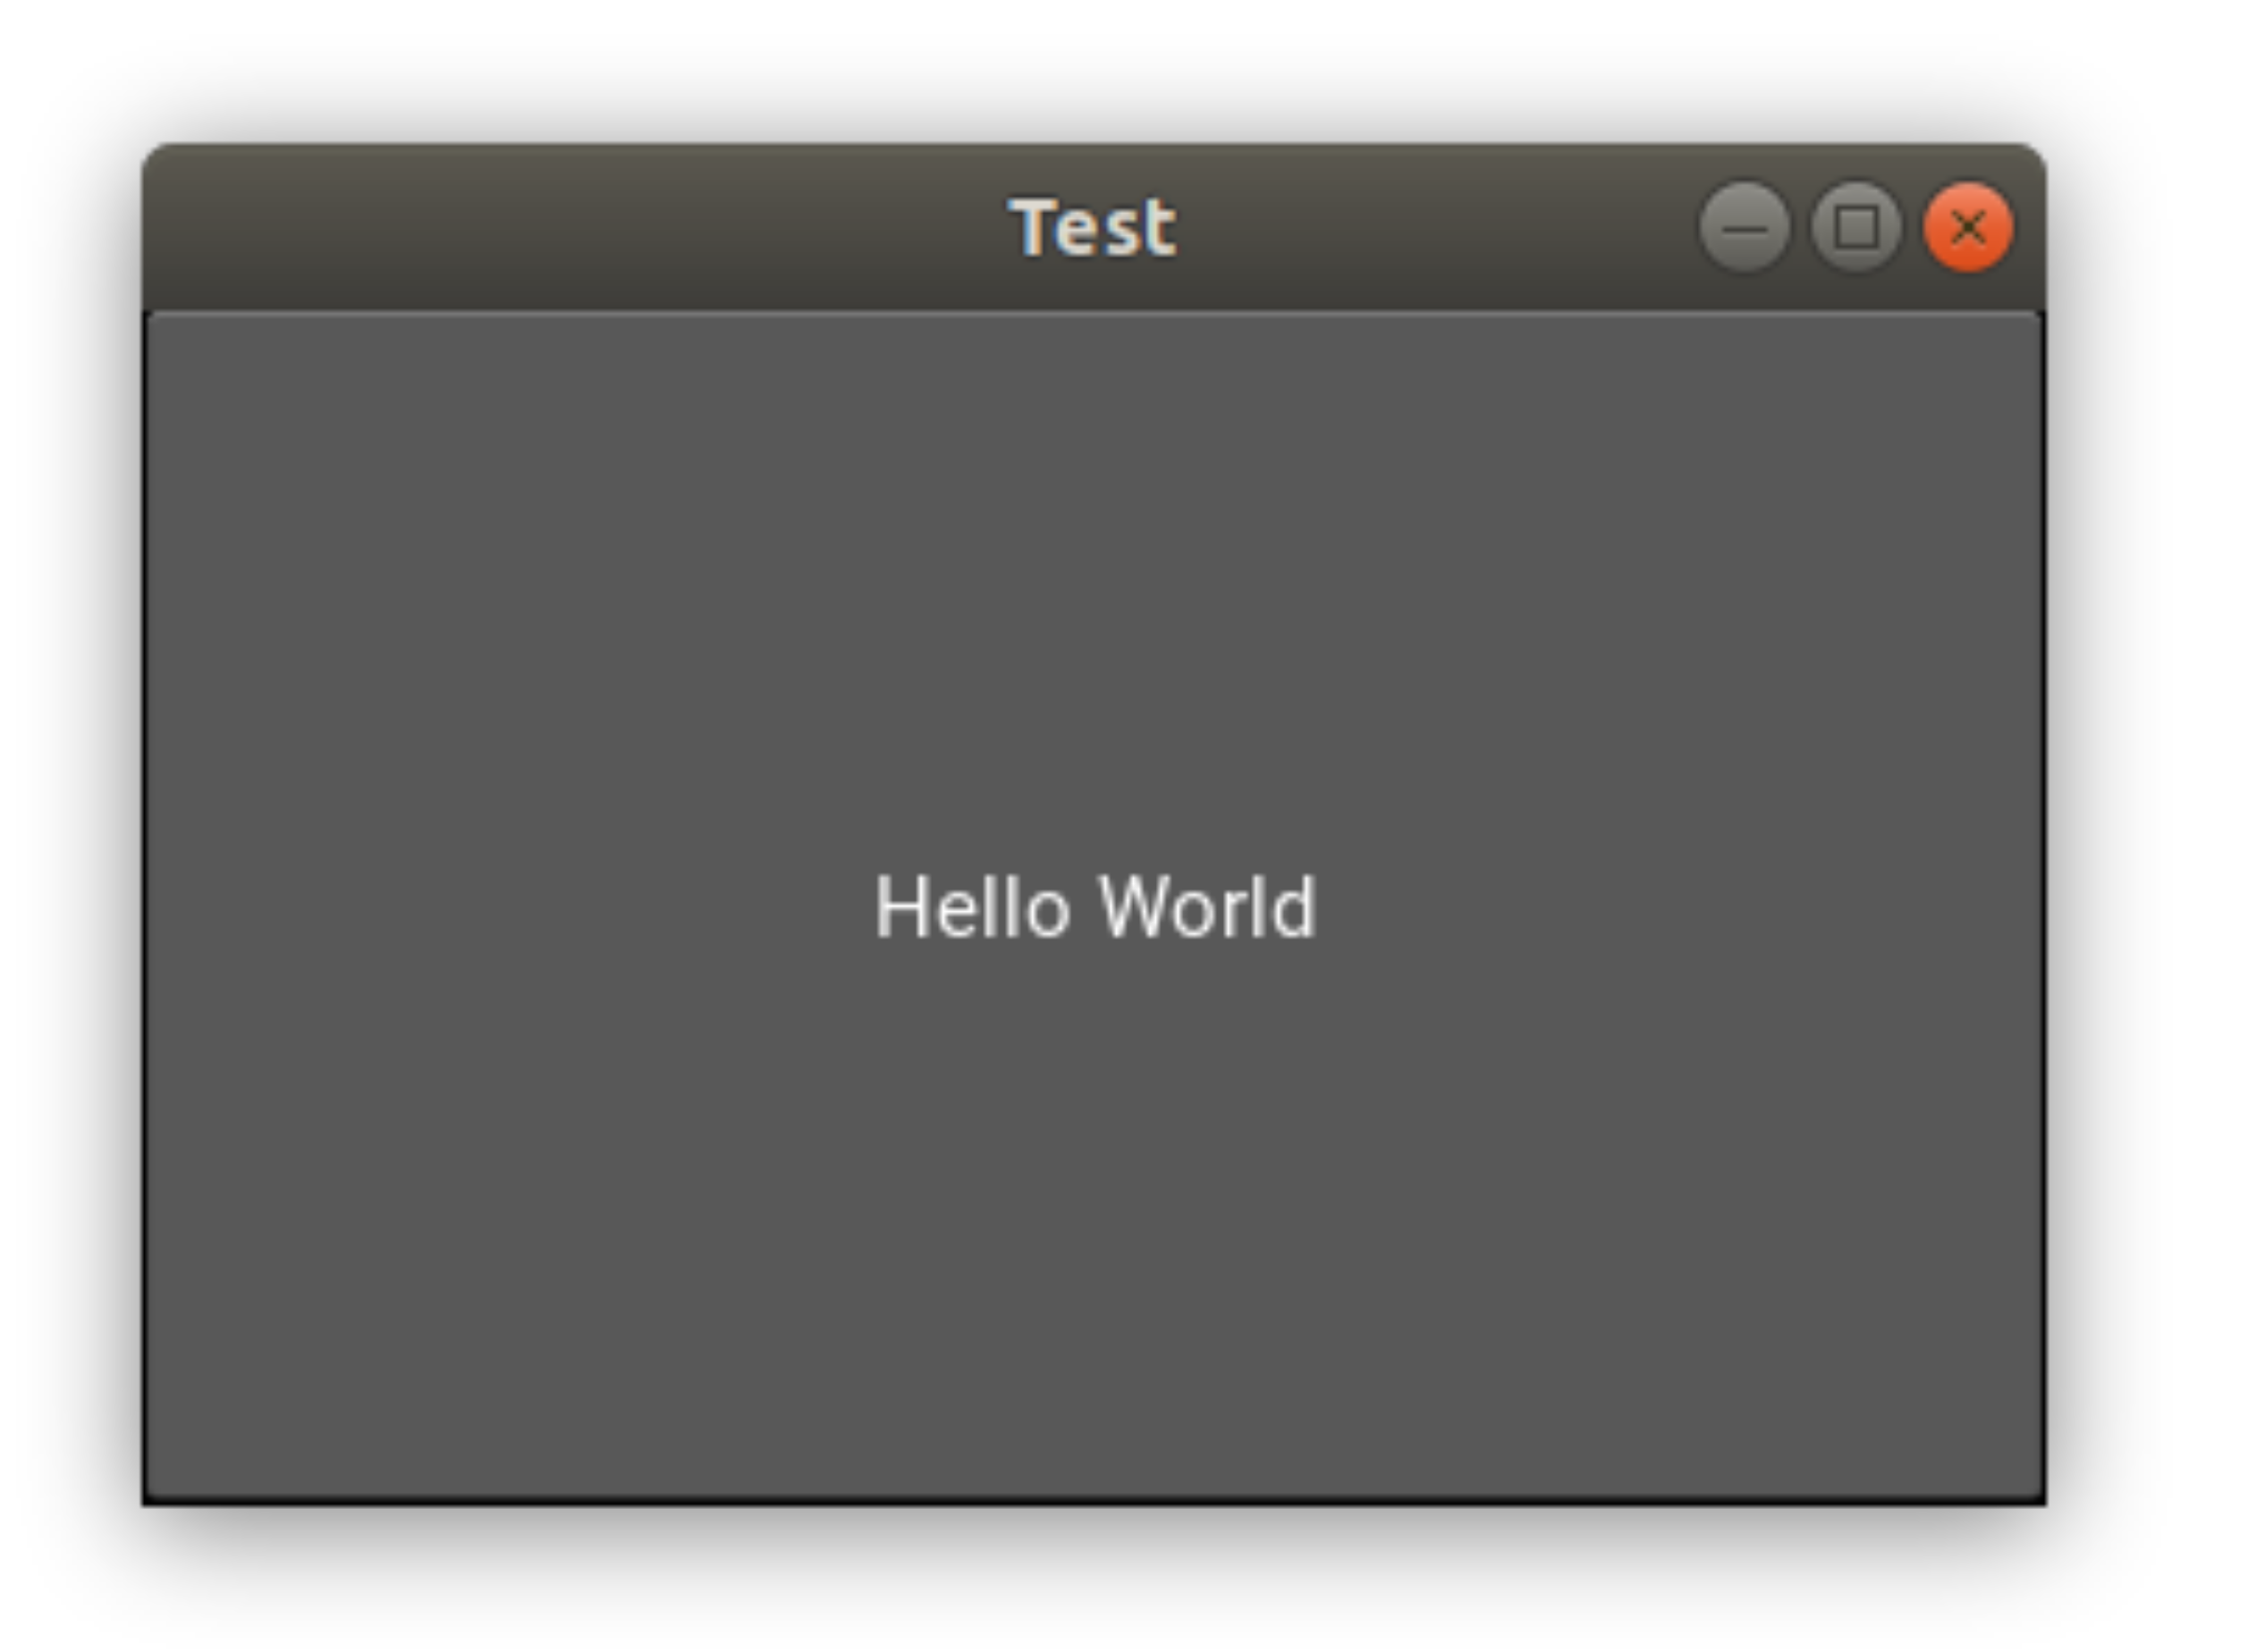
\includegraphics[width=7cm]{texto/fig/hello_world_kivy.png} 
                \end{center}
                \fonte{O Autor, 2018}
                \label{janela_kivy} 
            \end{figure}


            
            \subsubsection{SciPy, MatPlotLib, NumPy}
            \label{lim_scipy}
            
            SciPy é um ecossistema de ferramentas para processamento de dados científicos contando com ferramentes de manipulação de matrizes, plotagem de gráficos, interpolação dentro outras ferramentas \cite{scipy}.
            
            O ecossistema é de código aberto e as principais ferramentas são: NumPy para trabalhos com vetores e matrizes, MatPlotLib são ferramentas para plotagem de dados e o próprio SciPy para interpolação, cálculo de espectro de frequência dentre outras.
            
            A tabela \ref{pontos_ex_inter} apresenta 9 pontos distribuídos numa matriz quadrada de ordem 3, onde, a posição (2,2) possui uma anomalia, o código \ref{lim_scipy}.1 mostra como fazer a interpolação dos pontos e como plotar o resultado (figura \ref{fig_ex_inter}).
            
            \begin{table}[H]
                \centering
                \caption{Distribuição de pontos com valor anômalo ao centro.}
                \label{pontos_ex_inter}
                \resizebox{.22\textwidth}{!}{%
                \begin{tabular}{@{}cccl@{}}
                    \toprule
                    \textbf{Pontos}  & \textbf{x}   & \textbf{y}   & \textbf{z}  \\
                    \midrule
                        1&1       &   1     &  1     \\
                        %\hline
                        2&2       &   1     &  1     \\
                        %\hline
                        3&3       &   1     &  1     \\
                        %\hline
                        4&1       &   2     &  1     \\
                        %\hline
                        5&2       &   2     &  3     \\
                        %\hline
                        6&3       &   2     &  1     \\
                        %\hline
                        7&1       &   3     &  1     \\
                        %\hline
                        8&2       &   3     &  1     \\
                        %\hline
                        9&3       &   3     &  1     \\
                    \bottomrule
                \end{tabular}%
                }
                \fonte{O Autor, 2018}
            \end{table}
            

            Exemplo Numpy:
            \begin{quote}
             \codbox{\ini \cl{import} Numpy \cl{as} np        \\
                     \ini                                     \\
                     \ini  x = np.array([1,2,3,1,2,3,1,2,3])  \\
                     \ini  y = np.array([1,1,1,2,2,2,3,3,3])  \\
                     \ini  z = np.array([1,1,1,1,3,1,1,1,1])                                                                  
             }                                            \codnum{\ref{lim_scipy}.1}
            \end{quote}
            
            Exemplo SciPy:
            
            \begin{quote}
             \codbox{\ini \cl{from} scipy \cl{import} interpolate              \\
                     \ini \cl{from} scipy.interpolate \cl{import} griddata     \\
                     \ini                                                      \\
                     \ini  xi = np.arange(x.min(), x.max(), .01)               \\
                     \ini  yi = np.arange(y.min(), y.max(), .01)               \\
                     \ini  xi,yi = meshgrid(xi,yi)                             \\
                     \ini                                                      \\
                     \ini  \cc{ Interpolate}                                   \\
                     \ini  zi = griddata((x,y),z,(xi,yi),\ob{method}=\st{'cubic'})       
             }                                                                    \codnum{cont. \ref{lim_scipy}.1}
            \end{quote}
            
            Exemplo Matplotlib:
            
            \begin{quote}
             \codbox{\ini \cl{import} matplotlib.pyplot \cl{as} plt            \\
                     \ini                                                      \\
                     \ini  plt.figure(1)                                       \\
                     \ini  plt.subplot(111)                                    \\
                     \ini                                                      \\
                     \ini  zn = np.arange(z.min(), z.max() + 0.01, .01)        \\
                     \ini                                                      \\
                     \ini  plt.plot(x, y, \st{'kx'})                           \\
                     \ini  plt.contourf(xi, yi, zi, zn)                        \\
                     \ini  plt.colorbar()                                      \\ 
                     \ini  plt.grid()                                          \\
                     \ini  plt.set\_cmap(\st{'jet'})                           \\
                     \ini  plt.show()                                          \\
             }                                                                   \codnum{cont. \ref{lim_scipy}.1}
            \end{quote}
            
            \begin{figure}[H]
                \caption{Exemplo dos pontos interpolados usando SciPy e plotados usando MatPlotLib}
                \begin{center}
                    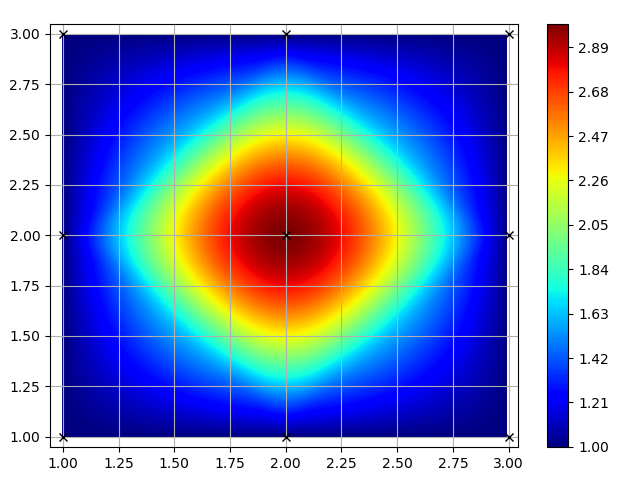
\includegraphics[width=10cm]{texto/fig/plot_ex.png} 
                \end{center}
                \fonte{O Autor, 2018}
                \label{fig_ex_inter} 
            \end{figure}
            
            
        \subsection{Pacotes de Processamentos do grupo Geoma - INPE}
    
        
    

	


% CAPITULO 3 ===================================================================================================================
	\chapter{Algoritmos e Processamentos}
\label{cap-areadeestudo}



	

% CAPITULO 4 ===================================================================================================================
	% RESULTADOR ESPERADOS
\chapter{Resultados Esperados}
    \label{cap-resultados}
    Espera-se ao final desse trabalho de conclusão de curso criar um programa para processamento do método \MT, escrito em Python e de fácil usabilidade.
    
    Também melhorar a compatibilidade com os diversos sistemas operacionais e distribuir sobre a licença de \en{software livre} para a comunidade geofísica, possibilitando a expansão no \MT na acadêmica visto que qualquer pessoa terá acesso ao programa.
    
    Ao final comparar os resultados obtidos com o programa em relação a forma que vinha sendo trabalho até então, as principais comparações serão: tempo de processamento, visualização, tempo de aprendizagem para uso da plataforma, coerência entre resultados e manipulação da forma de visualização. 
    
    

	

% CAPITULO 5 ===================================================================================================================
	% CRONOGRAMA

\chapter{Cronograma de Atividades}
    \label{cap-cronograma}

    \section{1º Semestre}
    
    \begin{table}[H]
                \centering
                \caption{Cronograma - 1º Semestre 2018}
                
                \resizebox{\textwidth}{!}{%
                \begin{tabular}{@{}lccccccl@{}}
                    \toprule
                    \textbf{Tarefa}  & {\bf Jan}& {\bf Fev}& {\bf Mar}& {\bf Abr}& {\bf Mai}& {\bf Jun} &  \\
                    \midrule
                       
                        {\bf 1.} Revisão Bibliográfica 		& 	X  & 	      & 	 & 	    & 	       & 	  \\ 
    
                        {\bf 1.1} Magnetotelúrico      		& 	X  & 	X     & X        & 	    & 	       & 	  \\ 
                        %\hline
                        {\bf 1.2} Python 3.5           		& 	   &          & X	 &X 	    & 	       & 	  \\ 
                        %\hline
                        %\hline
                        {\bf 1.3} Pacote PROC-MT (INPE)           	& 	   & 	      & 	 & 	    & X	       & X	  \\ 

                    \bottomrule
                \end{tabular}%
                }
                \fonte{O Autor, 2018}
            \end{table}
    
    
    
    \section{2º Semestre}
    
    
    \begin{table}[H]
                \centering
                \caption{Cronograma - 2º Semestre 2018}
                
                \resizebox{\textwidth}{!}{%
                \begin{tabular}{@{}lccccccl@{}}
                    \toprule
                    \textbf{Tarefa}  & {\bf Jul}& {\bf Ago}& {\bf Set}& {\bf Out}& {\bf Nov}& {\bf Dez} &  \\
                    \midrule
                       
                        {\bf 1.} Construção da Interface Gráfica 	 &X 	    & X	       & 	  & 	     & 	        & 	   \\ 
  
                        {\bf 2.} Desenvolvimento dos Scripts         & 	    & 	       & X	  & 	     & 	        & 	   \\ 
    
                        {\bf 3.} Fase de testes com Dados Sintéticos & 	    & 	       & 	  & X	     & 	        & 	   \\ 
    
                        {\bf 4.} Fase de testes com Dados Reais      & 	    & 	       & 	  & 	     &X	        & 	   \\ 
    
                        {\bf 5.} Liberação do Código                 & 	    & 	       & 	  & 	     & 	        & X	   \\ 
    
                    \bottomrule
                \end{tabular}%
                }
                \fonte{O Autor, 2018}
            \end{table}



% CAPITULO 6 ===================================================================================================================
	%\chapter{Materiais e métodos}
\label{cap-matemet}






% CAPITULO 7 ===================================================================================================================
	%\chapter{Planejamento}
\label{cap-planejamento}


\section{Fluxograma}
\label{cap-fluxograma}



\section{Cronograma}
\label{cap-cronograma}






% CAPITULO 8 ===================================================================================================================
	%\chapter{Resultados esperados}
\label{cap-resultadosesperados}




% CAPITULO 9 ===================================================================================================================
	%\chapter{Exemplo de Inserção de Figuras}
\label{cap-Figuras}

% % % % % % % % % % % % % % % % % % % % % % % % % % % % % % % % % % % % % % % % % % % % % %
% Incluir figuras no LaTeX não se dá por apenas copiar e colar, porém o processo é        %
% tão simples quanto. Use o ambiente figure demonstrado abaixo sempre que for necessário  %
% incluir uma imagem. Trocando apenas a localização/nome da imagem. O comando [h] na      %
% frente do ambiente é para que a imagem apareça o mais rápido possível no texto          %
% % % % % % % % % % % % % % % % % % % % % % % % % % % % % % % % % % % % % % % % % % % % % %

\begin{figure}[h]
\centering

\includegraphics[scale=0.5]{TEXTO/IMAGENS/nomedafigura.png}
\caption{}
\fonte{}
\end{figure}


% CAPITULO 10 ===================================================================================================================
	%\chapter{Exemplo de Tabela}
\label{cap-tabs}

% % % % % % % % % % % % % % % % % % % % % % % % % % % % % % % % % % % % % % % % % % % % 
% Para gerar tabelas mais facilmente utilize o site https://www.tablesgenerator.com/  %
% Porém para manter a configuração centralizada da tabela, copie do site apenas a     %
% partir de "\begin{tabular} até o final da tabela, NÃO SUBSTITUINDO o \end{tabular}%}%
% ou substitua porém lembre-se de incluir um %} ao final do comando.                  %
% % % % % % % % % % % % % % % % % % % % % % % % % % % % % % % % % % % % % % % % % % % % 

\begin{table}[h]
    \centering
    \caption{Exemplo de Tabela usando o Latex}
    \label{my-label}
    \resizebox{\textwidth}{!}{%
    \begin{tabular}{@{}ccccl@{}}
        \toprule
        \textbf{Um}  & \textbf{Exemplo}   & \textbf{de}   & \textbf{Tabela} &  \\
        \midrule
        \begin{tabular}[c]{@{}c@{}}
            coluna1     \\
            linha1
        \end{tabular} & 
        
        \begin{tabular}[c]{@{}c@{}}
            coluna2     \\
            linha1
        \end{tabular} & 
        
        \begin{tabular}[c]{@{}c@{}}
            coluna3     \\
            linha1
        \end{tabular} &         x               &  \\
        
        \begin{tabular}[c]{@{}c@{}}
        coluna1     \\
        linha2
        \end{tabular} & {\color[HTML]{000000} \begin{tabular}[c]{@{}c@{}}coluna2\\ linha2\end{tabular}} & \begin{tabular}[c]{@{}c@{}}coluna3\\ linha2\end{tabular}                         & x               &  \\
\begin{tabular}[c]{@{}c@{}}coluna1\\ linha3\end{tabular} & \begin{tabular}[c]{@{}c@{}}coluna2\\ linha3\end{tabular}                        & {\color[HTML]{000000} \begin{tabular}[c]{@{}c@{}}coluna3\\ linha3\end{tabular}}  & x               &  \\ 
\bottomrule
\end{tabular}%
}
\fonte{autor.}
\end{table}



% CAPITULO 11 ===================================================================================================================

% ===================================================================================================================








% BIBLIOGRAFIA ===================================================================================================================
\bibliographystyle{abntex2-alf}
\bibliography{biblio.bib}
% ===================================================================================================================







% GLOSSARIO ===================================================================================================================

	%\chapter*{Glossário}
% =============================================================================================================================







% APENDICE ===================================================================================================================

%\appendix

	%\chapter{Nome do Apêndice}
		%Depois do termo ``appendix'', qualquer capítulo aparecerá na forma correta, com o termo ``Apêndice''. Use apêndices quando houver material produzido pelo autor que ajuda no entendimento do trabalho mas que não faz parte do texto principal. Modelos de questionários utilizados, código fonte de programas, partituras completas, provas de teoremas acessórias, etc.
% ===================================================================================================================








% ANEXO ======================================================================================================================
%\annex

	%\chapter{Nome do Anexo}
		%Depois do termo ``annex'', qualquer capítulo aparecerá na forma correta, com o termo ``Anexo'' no título. Use anexos quando se tratar de material não produzido pelo autor, mas necessário no entendimento do trabalho. Por exemplo, definições matemáticas, sintaxe formal de linguagens de programação, trechos de manuais, etc.
% ===============================================================================================================================






\end{document}
% =============================================================================================================================
